\section{Bedienungsanleitung}
\subsection{Hintergrundinformationen}
\FloatBarrier

\paragraph{Spielinteraktion}
\subparagraph{Selektierungsvorgang}
Um einen gew"unschten Domino zu selektieren, muss der Spieler auf einen der schwarzen Kaesten rechts neben dem angezeigten Domino per Mausklick ausw"ahlen (siehe Abbildung \ref{fig:erstesSelektierenNaechsteBank}). Anschlie"send erscheint die Zahl \emph{1} in diesem Feld. Diese Zahl repr"asentiert den menschlichen Spieler. Um dem Benutzer deutlich zu machen von welcher Bank, oder ob er "uberhaupt in seinem aktuellen Zug einen Domino selektieren darf, kann dieser nur auf der Bank, welche nicht verschwommen ist, einen Domino ausw"ahlen. Um jederzeit ablesen zu k"onnen welcher Spieler gerade am Zug ist, gibt es hierf"ur ein Feld oberhalb der Darstellung der beiden B"anke eine Anzeige. 

\begin{figure}
	\centering
	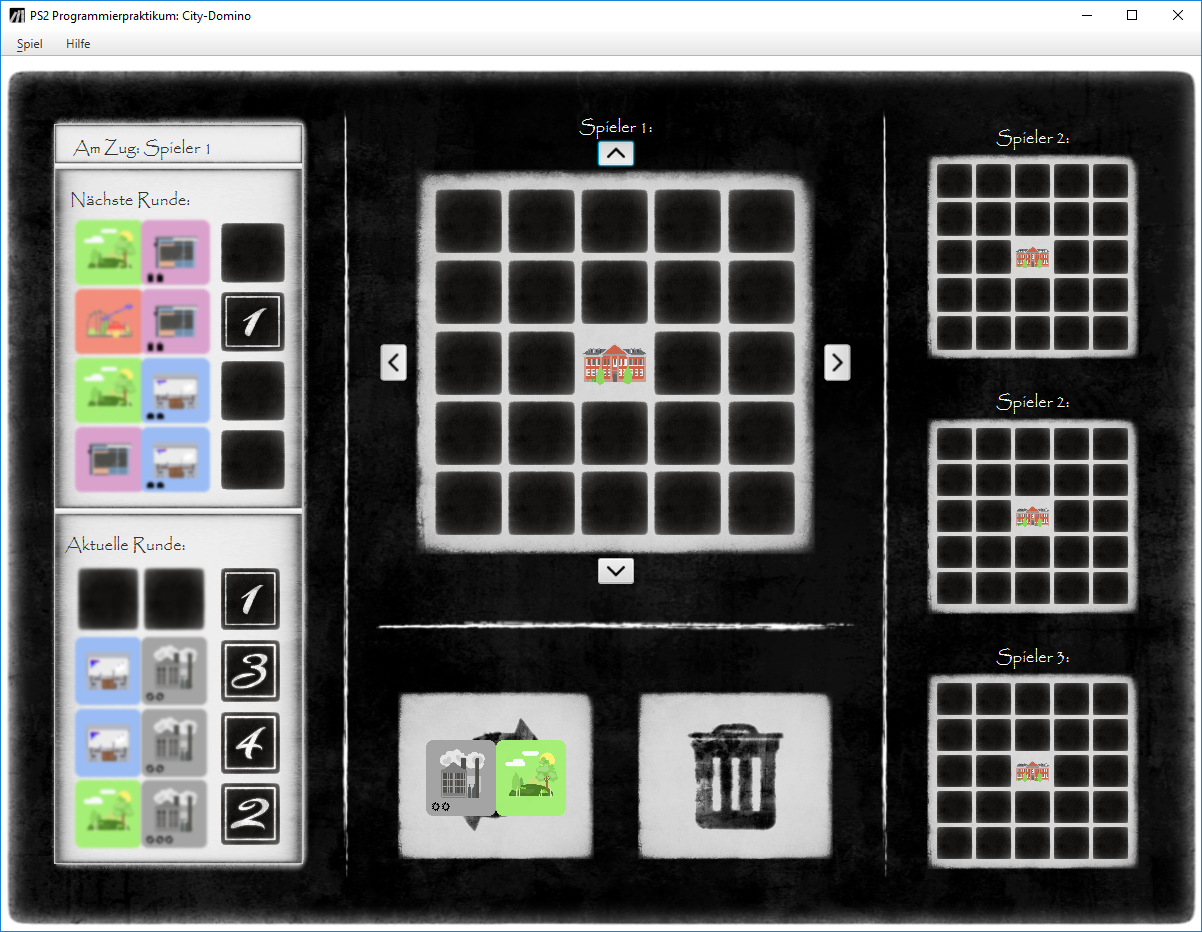
\includegraphics{screenshots/screenshot_ErstesSelektierenAufNaechsterBank}
	\caption[Erstes Selektieren]{Erstes Selektieren auf der Bank f"ur die n"achste Runde}
	\label{fig:erstesSelektierenNaechsteBank}
\end{figure}

\subparagraph{Justierung des Dominos}
Nachdem der Spieler erfolgreich s"amtliche Selektierungsschritte auf den beiden B"anken absolviert hat, kann er seinen zuvor ausgew"ahlten Domino in dem daf"ur vorgesehenen Kasten drehen. Um den Domino um 90 Grad zu drehen muss der Spieler lediglich einen Mausklick auf dem Domino ausf"uhren. 

\subparagraph{Positionierung auf dem Spielfeld}
Um den justierten Domino nun auf dem Feld zu platzieren, zieht der Benutzer den Domino an die gew"unschte Stelle auf dem Spielfeld. W"ahrend dem Ziehen f"arben sich die zugrunde liegenden Felder jeweils gr"un, falls es m"oglich sein sollte den Domino an der gew"unschten Stelle anzulegen (siehe Abbildung \pageref{fig:hovernGruen}), beziehungsweise rot, falls dies nicht der Fall sein sollte (siehe Abbildung \ref{fig:hovernRot}. F"ur genauere Informationen siehe Abschnitt \ref{par:anlegeregeln}). Falls der Domino an der gew"unschten Stelle nicht passen sollte und dennoch versucht wird ihn dort zu platzieren, passiert nichts. Der Domino befindet sich weiterhin in dem Kasten zum Justieren der Ausrichtung und es kann ein neuer Versuch unternommen werden. 

\subparagraph{Verwerfen des Dominos}
Um den Domino zu verwerfen reicht es per Mausklick einmal auf das M"ulleimer-Symbol rechts neben dem Domino zu klicken. Der Domino wird anschlie"send aus dem Rotationsfeld entfernt. 

\begin{figure}
	\centering
	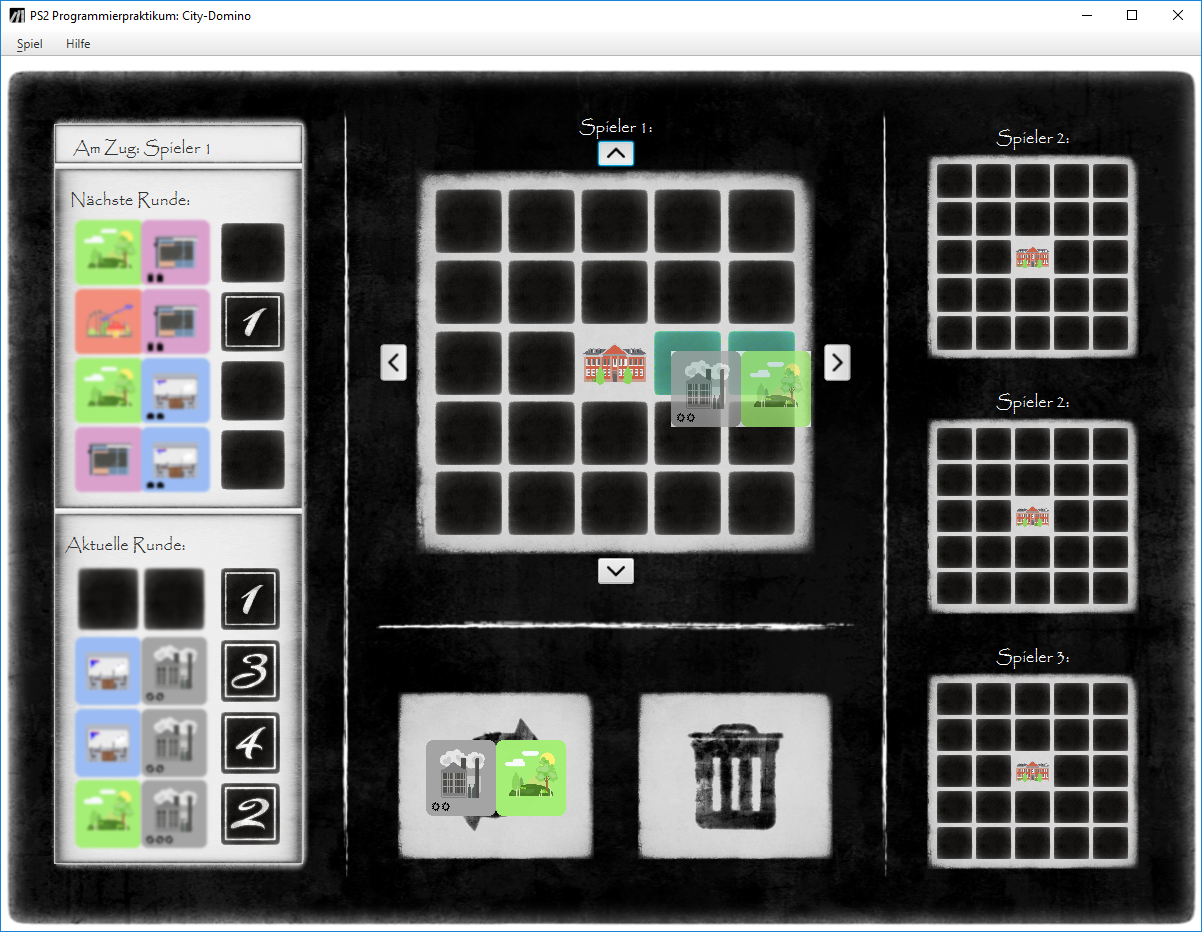
\includegraphics{screenshots/screenshot_HovernGruen}
	\caption{Schwebender Domino "uber g"ultiger Position}
	\label{fig:hovernGruen}
\end{figure}

\begin{figure}
	\centering
	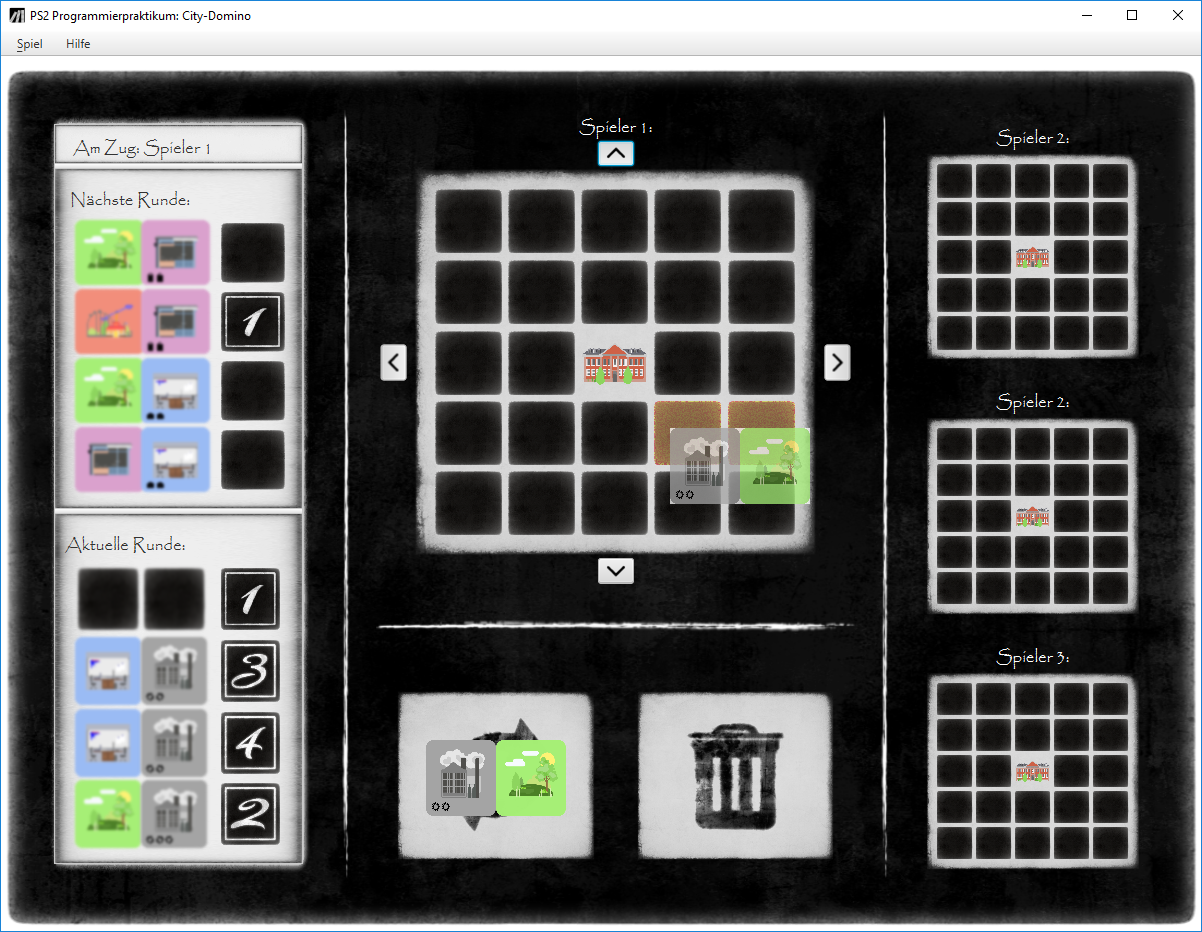
\includegraphics{screenshots/screenshot_HovernRot}
	\caption{Schwebender Domino "uber ung"ultiger Position}
	\label{fig:hovernRot}
\end{figure}


\newpage

\begin{figure}
	\centering
	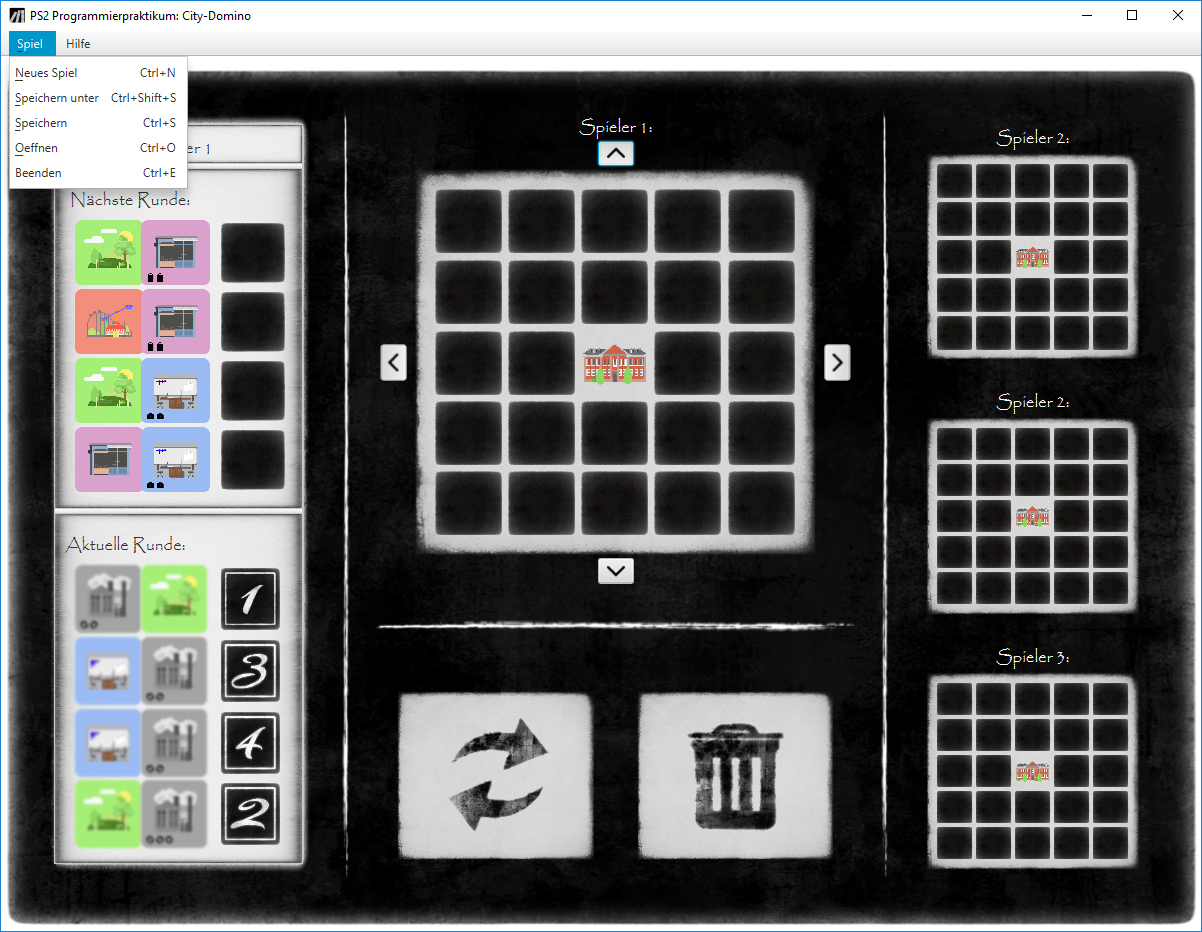
\includegraphics{screenshots/screenshot_Menue}
	\caption{Men"uoptionen}
	\label{fig:menueoptionen}
\end{figure}

\paragraph{Men"uinteraktion}
\subparagraph{Starten bzw. Schlie"sen}
Um ein neues Spiel zu starten w"ahlt der Benutzer den Men"upunkt "\emph{Neues Spiel}". Alternativ ist dies auch per Tastenkombination \verb|strg + N| m"oglich. Um das ge"offnete Fenster zu schlie"sen und das bestehende Spiel zu verwerfen, w"ahlt der Benutzer den Reiter \emph{Beenden} (Tastenkombination \verb|strg + E|). Falls der Benutzer das Spiel nicht vorher gespeichert hat erscheint hierbei ein weiteres Fenster, welches den Benutzer darauf hinweist und ihm die M"oglichkeit gibt dies nachzuholen (siehe folgenden Abschnitt). M"ochte er fortfahren, ohne den aktuellen Spielstand zu speichern, muss der Button mit der Aufschrift \emph{Abbrechen} bet"atigt werden (siehe Abbildung \ref{fig:nachtrSpeichern}). 

\begin{figure}
	\centering
	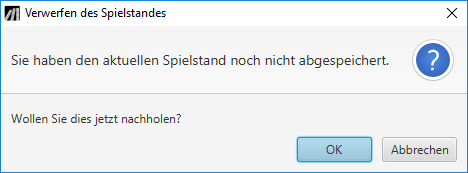
\includegraphics[width=.6\linewidth]{screenshots/screenshot_NachtraeglichesAbspeichern}
	\caption{Nachtr"agliches Abspeichern}
	\label{fig:nachtrSpeichern}
\end{figure}

\subparagraph{Spielstand abspeichern}
\label{spar:anleitung_speichern}
Um einen Spielstand zu speichern gibt es zwei Reiter mit folgenden M"oglichkeiten:
\begin{enumerate}
	\item Speichern: \verb|Strg + S|
	\item Speichern unter: \verb|Strg + Shift + S|
\end{enumerate}
\glqq \emph{Speichern unter}\grqq {} gibt dem Benutzer die M"oglichkeit, ausgehend vom Ablageverzeichnis, den gew"unschten Speicherort anzugeben. Hierzu navigiert er mit dem gegebenen Filechooser an den gew"unschten Speicherort und gibt der abzuspeichernden Datei einen Namen. Hierbei wurde die ben"otigte Dateiendung \emph{.txt} bereits ausgew"ahlt, sodass der Benutzer seine Auswahl lediglich auf dem Feld \emph{Speichern} per Mausklick zu best"atigen braucht (siehe Abbildung \ref{fig:filechooser}). 

Der Reiter \glqq \emph{Speichern}\grqq {} erm"oglicht es einen bereits gespeicherten Spielstand ohne "Offnen eines Filechoosers zu "uberschreiben. Falls der Benutzer diesen Reiter bet"atigt, ohne dass zuvor ein Spielstand des aktuellen Spiels abgespeichert worden ist, "offnet sich bei der Auswahl dieses Reiters dennoch ein Filechooser und es wird nach der Funktionsweise von \glqq \emph{Speichern unter}\grqq {} vorgegangen.

\subparagraph{"Offnen}
"Ahnlich wie beim Reiter \glqq \emph{Speichern unter}\grqq {} wird hier ein Filechooser ge"offnet. Dieser wird jedoch dazu verwendet eine Datei auszuw"ahlen um aus dieser einen Spielstand zu lesen. Falls die Datei nicht der geforderten Syntax entspricht, erscheint eine Fehlermeldung in Form eines Popup-Fensters mit dem einer groben Fehlermeldung wo der Fehler liegt \lstref{fig:Fehleruebersicht}. Falls der Benutzer vor dem "Offnen eines neuen Spielstands den alten nicht gespeichert hat, wird er "ahnlich wie beim Beenden darauf hingewiesen und es wird per Filechooser eine M"oglichkeit bereitgestellt dies nachzuholen. Falls eine fehlerhafte Datei ge"offnet wurde, wird dies dem Benutzer wieder per Pop-Up-Fenster mitgeteilt. Allerdings muss anschlie"send ein valides Spiel ge"offnet oder ein neues Spiel gestartet werden. Der Benutzer kann also nicht einfach das gerade laufende Spiel weiterspielen. 

\begin{figure}
	\centering
	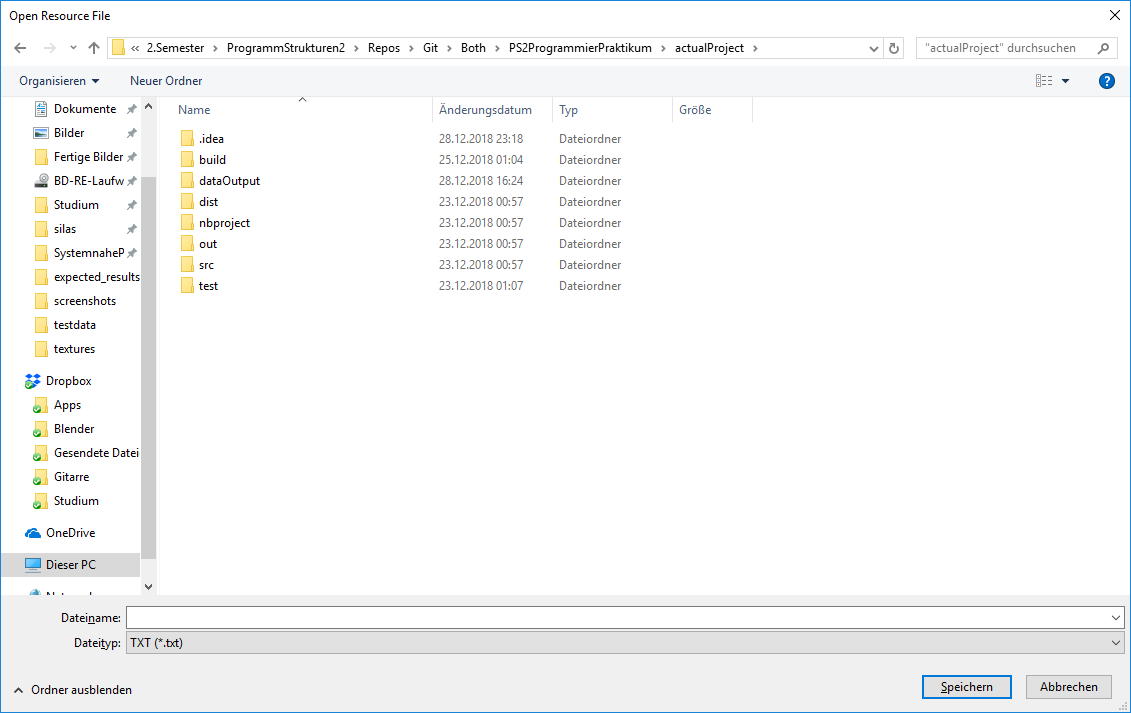
\includegraphics{screenshots/screenshot_Filechooser}
	\caption[Filechooser]{Filechooser zum Abspeichern eines Spielstandes}
	\label{fig:filechooser}
\end{figure}

\begin{figure*}
        \centering
        \begin{subfigure}[b]{0.35\textwidth}   
            \centering 
            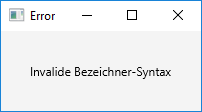
\includegraphics[width=\textwidth]{screenshots/screenshot_ErrorBezeichner}
            \caption[]%
            {{\small Bezeichner}}    
            \label{fig:BezeichnerErr}
        \end{subfigure}
        \quad
        \begin{subfigure}[b]{0.35\textwidth}   
            \centering 
            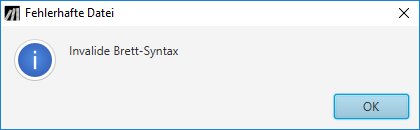
\includegraphics[width=\textwidth]{screenshots/screenshot_ErrorBrett}
            \caption[]%
            {{\small Brett}}    
            \label{fig:BrettErr}
        \end{subfigure}
        \vskip\baselineskip
        \begin{subfigure}[b]{0.35\textwidth}   
            \centering 
            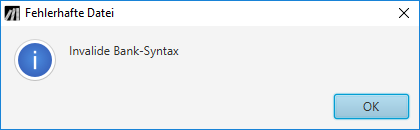
\includegraphics[width=\textwidth]{screenshots/screenshot_ErrorBank}
            \caption[]%
            {{\small Bank}}    
            \label{fig:BankErr}
        \end{subfigure}
        \quad
        \begin{subfigure}[b]{0.35\textwidth}   
            \centering 
            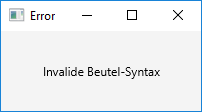
\includegraphics[width=\textwidth]{screenshots/screenshot_ErrorBeutel}
            \caption[]%
            {{\small Beutel}}    
            \label{fig:BeutelErr}
        \end{subfigure}
        \caption
        {\small Unterschiedliche Fehlermeldungen beim Einlesen einer Datei} 
        \label{fig:Fehleruebersicht}
    \end{figure*}

\subparagraph{Hilfestellung}
Unter dem Reiter \glqq \emph{Hilfe}\grqq {} ist der Link zur Website der Aufgabenstellung zu finden. Beim Ausw"ahlen des Men"upunktes \emph{Aufgabenstellung} "offnet sich diese im, vom Benutzer standardm"a"sig genutzten, Browser. 


\subsection{Programmfunktionalit"at}
Generell gilt es zwischen einem standardm"a"sig ausgef"uhrten Spiel und einem aus einer Datei eingelesenem Spiel zu unterscheiden. 

\paragraph{Spiel ohne Einlesen einer Datei}
\subparagraph{Spielbeginn}
\emph{Ein Spielbeutel für alle Spieler enthält 48 Spielkarten in der Größe von zwei Zellen, die auf ihren zwei Hälften jeweils einen (evtl. auch den gleichen) Stadtteiltyp anzeigen. Die Stadtteiltypen unterscheiden sich durch Bild und Hintergrundfarbe voneinander. Jede Spielkarte besitzt eine definierte Wertigkeit. Auf manchen Stadtteilen sind zusätzlich ein bis drei Prestigesymbole abgebildet. Jeder Spieler besitzt ein eigenes 5*5-Zellen großes Spielfeld und legt zu Beginn sein Stadtzentrum mittig ab}
\cite{aufgabenstellung}. 
(siehe Abbildung \ref{fig:spielbeginnGui}). Dies wird bereits vom Spiel "ubernommen, sodass der erste Spielzug des Benutzers das initiales Selektieren vom ersten Auswahlbereich (hier mit \emph{Aktuelle Runde} gekennzeichnet) darstellt. Um einen Domino selektieren zu k"onnen \emph{werden vier Karten gezogen und im ersten Auswahlbereich angezeigt. Dabei wird die niederwertigste Karte zuoberst, die höchstwertigste zuunterst einsortiert. Der erste Spieler markiert die Karte im Auswahlbereich, die er gerne nehmen würde, die anderen Spieler treffen ihre Auswahl der Reihe nach ebenfalls und markieren die jeweils gewünschte Karte. Wurden alle Karten markiert, dann werden wieder vier Karten gezogen und ebenso sortiert im zweiten Auswahlbereich angezeigt.} 
\cite{aufgabenstellung}
(Siehe Abbildung \ref{fig:initialesSelektierenOben})

\begin{figure}
	\centering
	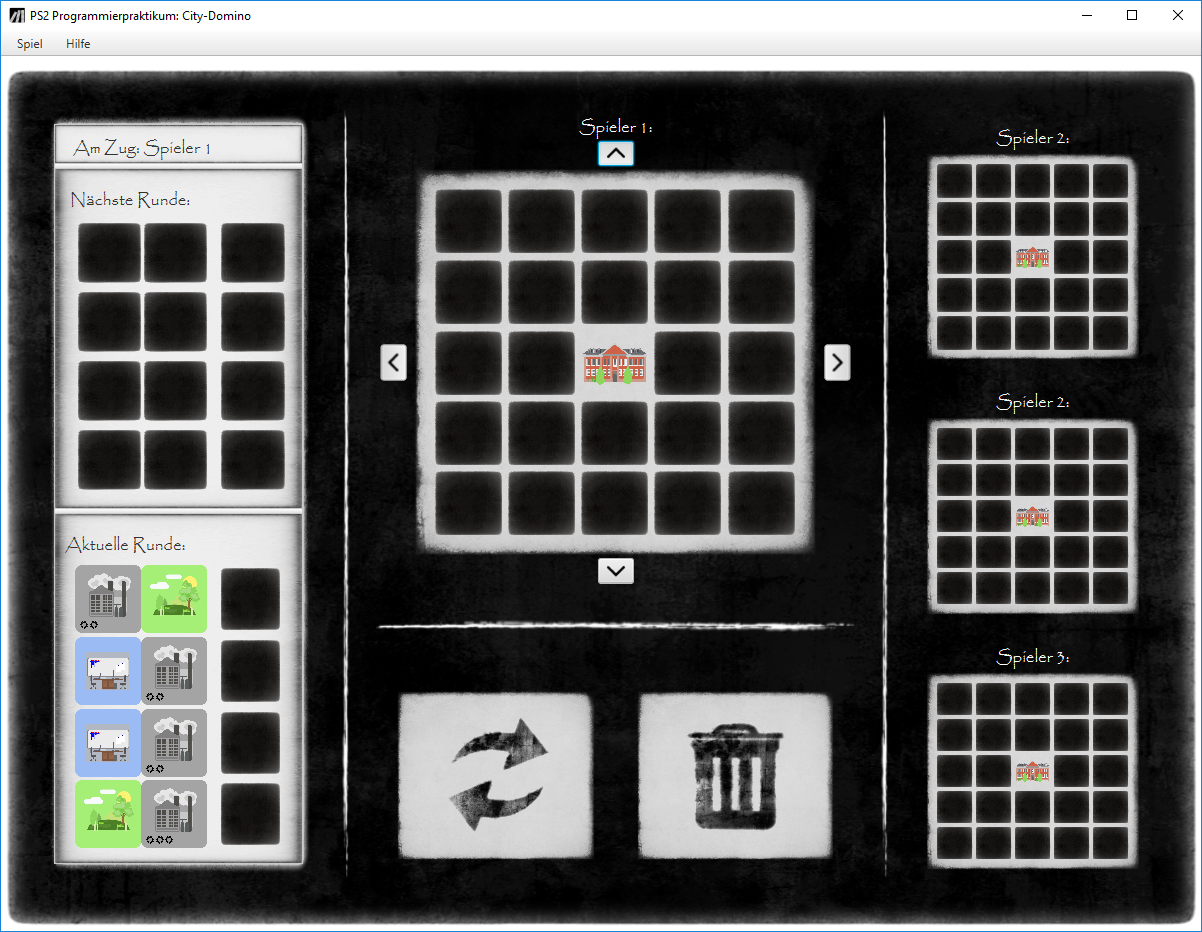
\includegraphics{screenshots/screenshot_Spielbeginn.png}
	\caption[Spielbeginn]{Spielbeginn nach Programmstart}
	\label{fig:spielbeginnGui}
\end{figure}

\begin{figure}
	\centering
	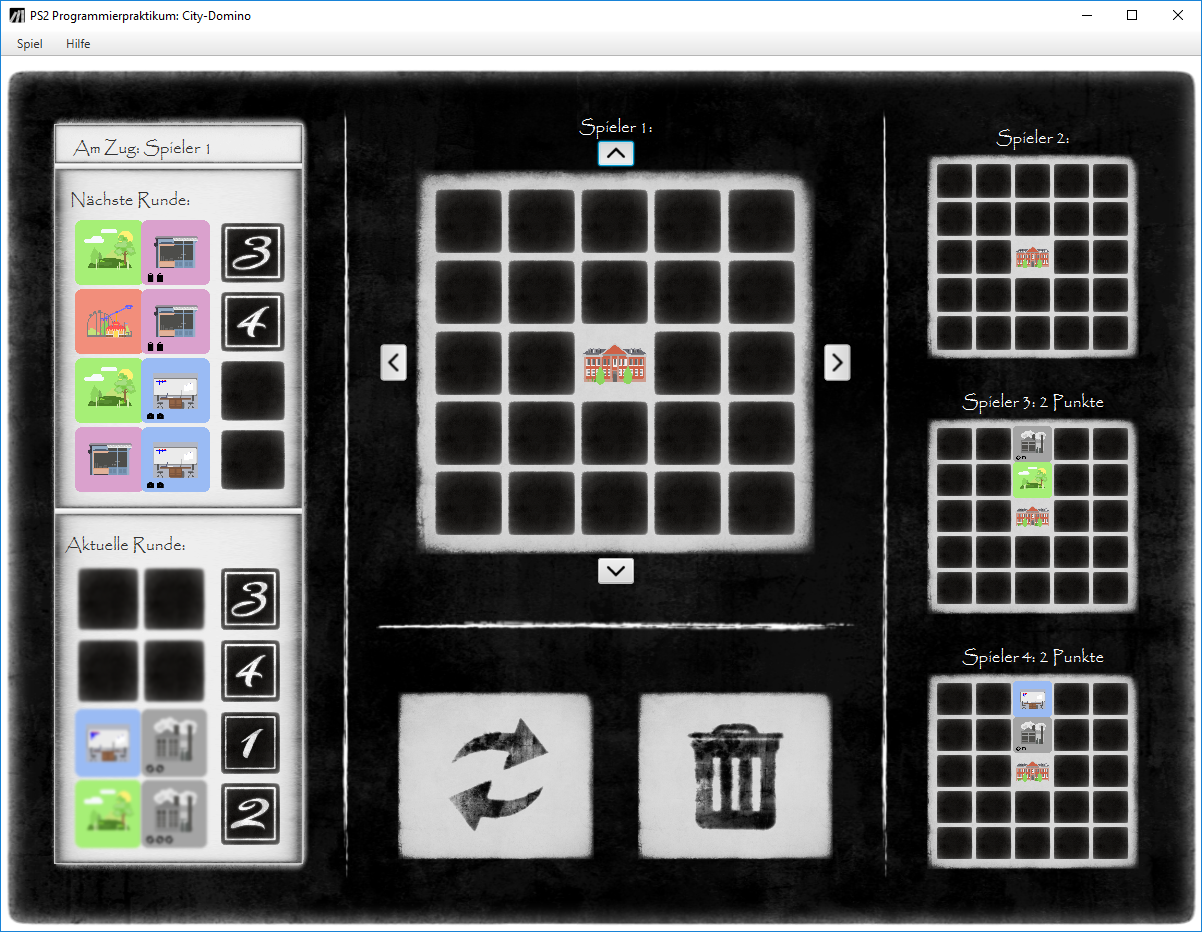
\includegraphics{screenshots/screenshot_InitialesSelektieren2.png}
	\caption[Initiales Selektieren - oben]{Initiales Selektieren (oben) nach Programmstart}
	\label{fig:initialesSelektierenOben}
\end{figure}

\subparagraph{Spielablauf}
\emph{Derjenige, der die oberste Karte im ersten Auswahlbereich markiert hat, beginnt eine Runde, es folgen der Reihe
nach die Spieler, die die jeweils darunterliegende Karte markiert haben. In einer Runde wird zunächst eine Karte
aus dem zweiten Auswahlbereich markiert und dadurch für die kommende Runde gewählt. Je wertvoller also seine
markierte Karte in dieser Runde ist, desto später ist der Spieler am Zug und desto weniger Auswahl hat er für die
kommende Runde.}
\cite{aufgabenstellung}
Zwischen dem initialen Selektieren und dem beschriebenen Spielablauf gibt es keine Pause. Wie man in Abbildung \ref{fig:initialesSelektierenMittig} sehen kann, ziehen die Gegner bereits ihre ersten Dominos auf ihr Feld, obwohl der Benutzer noch gar nicht an der Reihe war. Nun kann der Benutzer einen Domino auf dem n"achsten Auswahlstapel beziehungsweise der n"achsten Bank einen der "ubrig gebliebenen Dominosteine ausw"ahlen. Nun wird der Domino, welcher als erstes selektiert wurde, in den Kasten zum Rotieren geladen (siehe Abbildung \ref{fig:erstesRotieren}). Der Benutzer kann nun den Stein auf sein Brett legen (Abbildung \ref{fig:ersteAblage}). Nach dieser Aktion selektiert der Benutzer einen Domino auf der Bank f"ur die n"achste Runde. Danach muss er wieder "warten" bis er an der Reihe ist um einen ausgew"ahlten Domino auf seinem Brett zu platzieren. Alternativ kann er seinen Domino aber auch verwerfen.

\begin{figure}
	\centering
	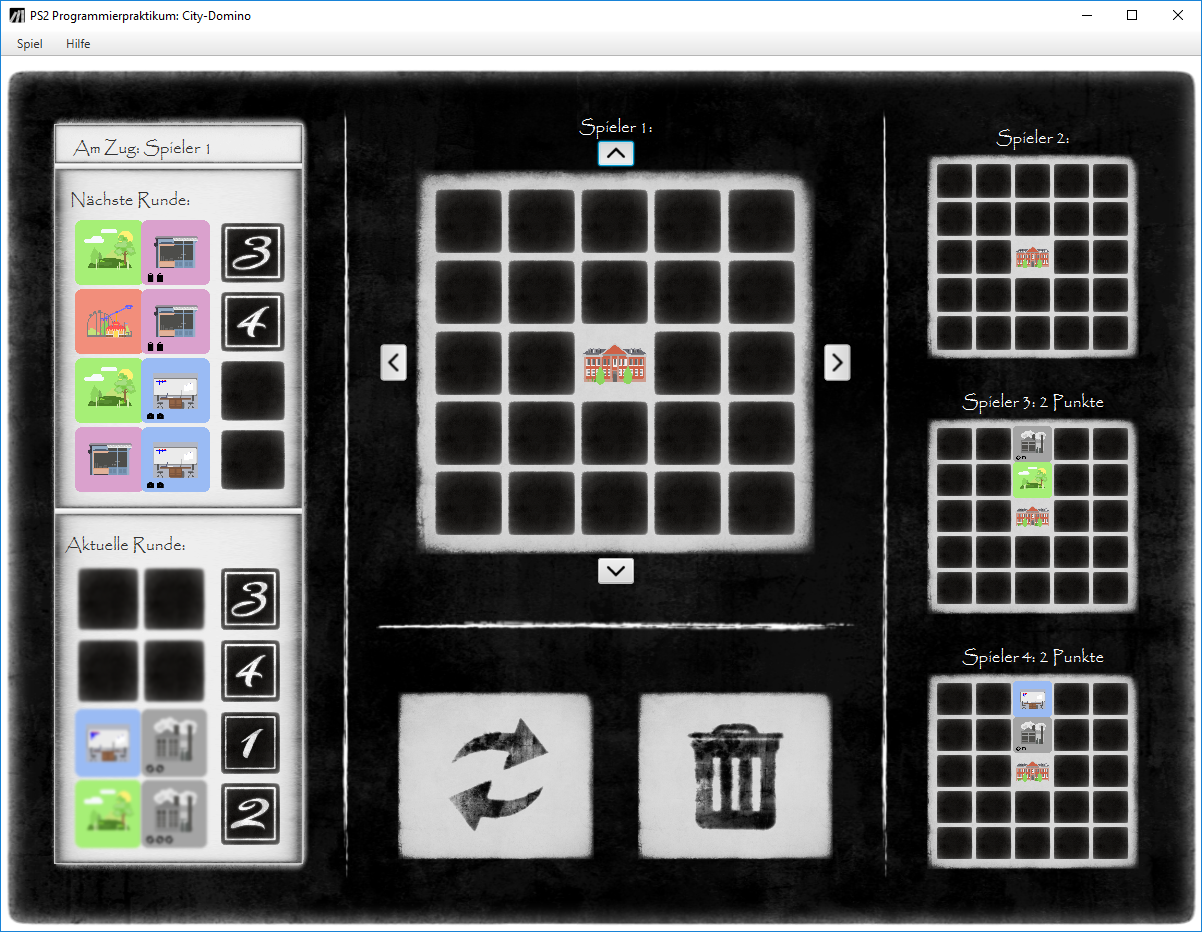
\includegraphics{screenshots/screenshot_InitialesSelektieren2.png}
	\caption[Initiales Selektieren - mittig]{Initiales Selektieren (mittig) nach Programmstart}
	\label{fig:initialesSelektierenMittig}
\end{figure}

\begin{figure}
	\centering
	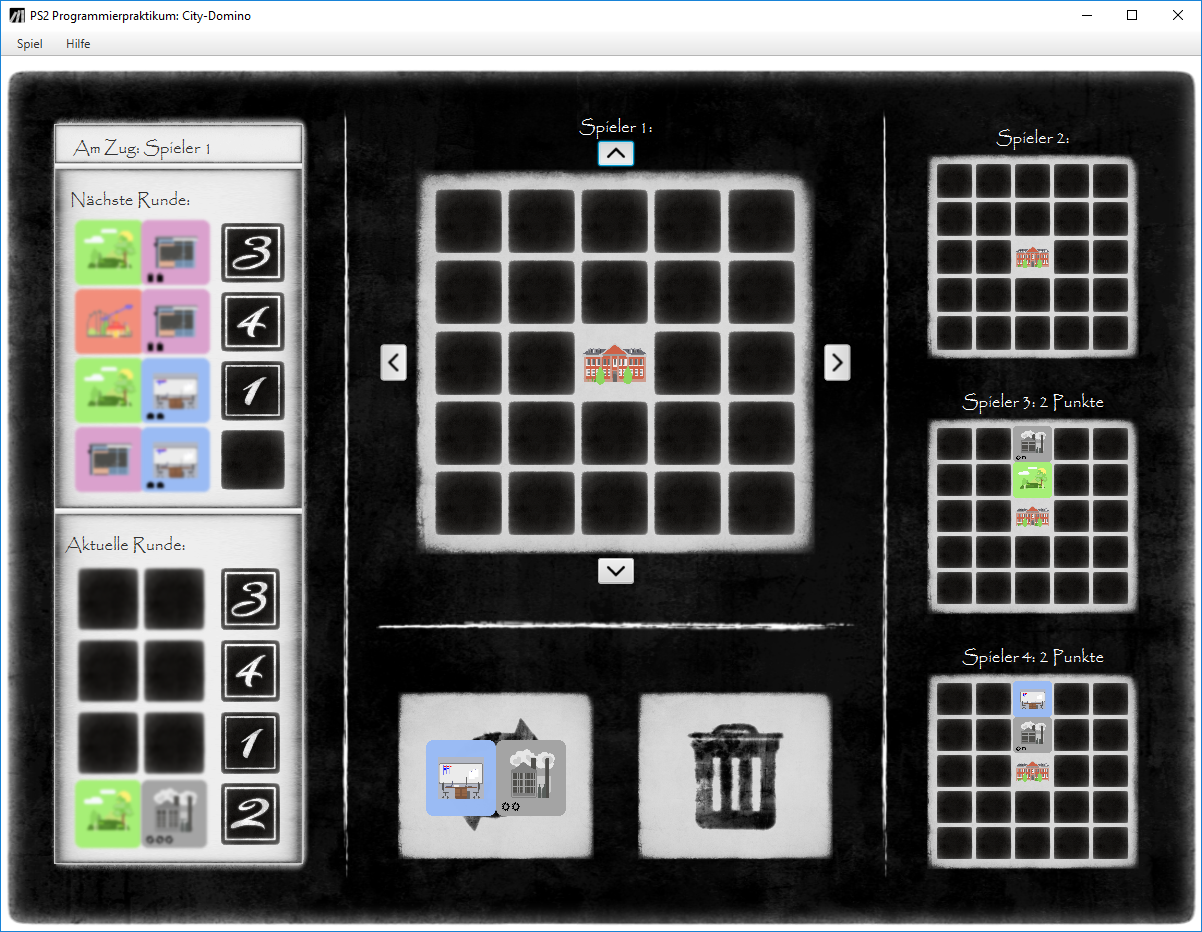
\includegraphics{screenshots/screenshot_ErstesRotieren.png}
	\caption{Erstes Rotieren}
	\label{fig:erstesRotieren}
\end{figure}

\begin{figure}
	\centering
	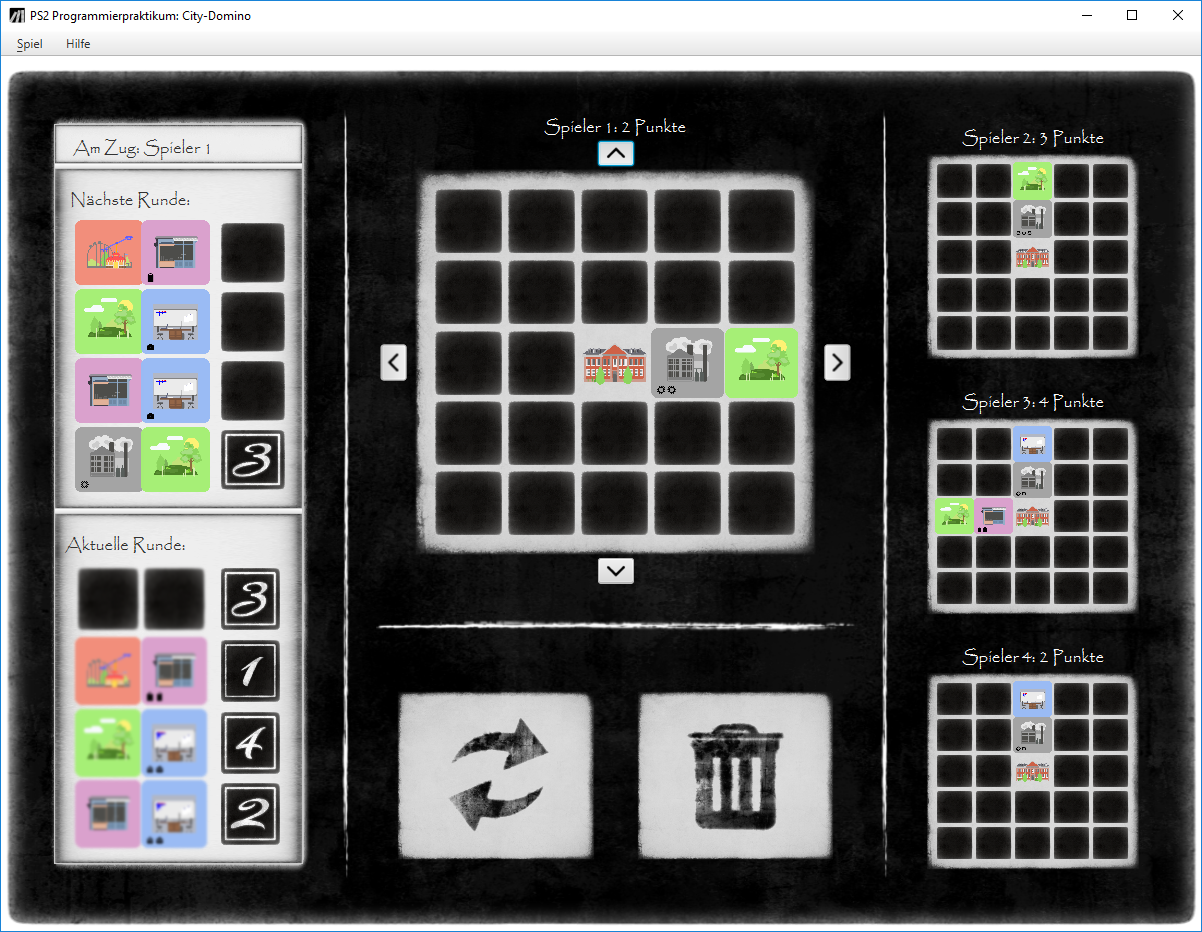
\includegraphics{screenshots/screenshot_ErsteAblage.png}
	\caption[Erste Ablage]{Erste Ablage auf dem Spielfeld}
	\label{fig:ersteAblage}
\end{figure}

\paragraph{Einlesen einer Datei}
Nachdem der Benutzer eine Datei eingelesen hat, ist dieser auch gleichzeitig am Zug. Je nachdem, ob der Spielstand w"ahrend des initialen Selektierens oder w"ahrend einer standardm"a"sigen Runde abgespeichert wurde, muss der Benutzer entweder von der Bank der aktuellen Runde oder von der Bank der n"achsten Runde selektieren. Generell gelten hier die gleichen Regeln zum Spielablauf wie beim Spielen ohne gespeicherten Spielstand, allerdings kann hierbei der Schritt des initialen Selektierens "ubersprungen werden. 

\paragraph{Anlegeregeln}
\label{par:anlegeregeln}
\emph{Die erste Karte muss an das Stadtzentrum angrenzen. An das Stadtzentrum darf jeder Stadtteil angrenzen. Legt man eine Karte an eine andere Karte an, so muss mindestens eine Hälfte mit einer Seite an einen identischen Stadtteiltyp einer liegenden Karte angrenzen. Passt die abzulegende Karte weder an das Stadtzentrum noch an eine bereits ausliegende Karte, so wird sie verworfen. Alle Spielkarten müssen in das 5*5-Feld passen, keine Hälfte darf hinausragen. Das Stadtzentrum muss aber nicht in der Mitte liegen, sondern kann im Spielverlauf verschoben werden, wodurch sich alle bereits gelegten Karten mit verschieben. Eine abgelegte Karte kann nicht verschoben werden.}
\cite{aufgabenstellung}

\paragraph{Spielende}
\emph{Wurden alle Spielkarten aus dem Beutel gezogen und von den
Auswahlbereichen auf die Spielfelder platziert bzw. verworfen, werden die
Punkte ermittelt.
\begin{itemize}
	\item Jede Stadt besteht aus mehreren Stadtteilen. Ein Stadtteil setzt sich aus waagerecht und/oder senkrecht verbundenen Zellen desselben Stadtteiltyps zusammen. Das Stadtzentrum zählt zu keinem Stadtteil dazu.
	\item Die Punkte eines Stadtteils ergeben sich aus der Anzahl seiner Zellen
multipliziert mit der Anzahl darin enthaltener Prestigesymbole.
	\item Innerhalb einer Stadt kann es mehrere voneinander getrennte Stadtteile
desselben Typs geben. Jeder Stadtteil ist einzeln auszuwerten. Stadtteile ohne Prestigesymbole bringen keine Punkte. 
\end{itemize}
Für die Auswertung wird für jeden Spieler die Summe der Punkte seiner Gebiete ermittelt. Gewonnen hat der Spieler mit den meisten Punkten. Bei einem Gleichstand gewinnt der Spieler mit dem größten einzelnen Gebiet. Besteht auch hier Gleichstand, so siegen beide Spieler gleichermaßen.
}
\cite{aufgabenstellung}
